\documentclass[12pt,a4paper]{article}
\usepackage{geometry}
%\setlength{\parindent}{0pt}
\usepackage{amssymb}
\usepackage{amsmath}
\usepackage{amsthm}
\usepackage{sectsty}
\usepackage{graphicx}
\usepackage[square,numbers]{natbib}
\usepackage[russian,english]{babel}
\usepackage[T2A]{fontenc}
\usepackage[utf8]{inputenc}
\usepackage{caption}
\usepackage{subcaption}
\usepackage[hidelinks]{hyperref}
\usepackage[table]{xcolor}
\usepackage{booktabs}

\geometry{top=2cm}
\geometry{bottom=2cm}
\geometry{left=2cm}
\geometry{right=2cm}
\geometry{bindingoffset=0cm}

\bibliographystyle{abbrvnat}
%\subsectionfont{\normalfont\itshape}

%\theoremstyle{definition}
\newtheorem{definition}{Definition}[section]
\newtheorem{theorem}{Theorem}[section]

\DeclareMathOperator{\Var}{Var}
\DeclareMathOperator{\VaR}{VaR_\alpha}

\title{Probabilistic Multivariate Time Series Forecasting using Deep Generative Models}
\date{\today}

\author{
    \small Vitaliy Pozdnyakov \\
    \small Faculty of Computer Science \\
    \small \textit{National Research University Higher School of Economics} \\
    \small Moscow, Russia\\
    }

\begin{document}

\selectlanguage{english} 
\begin{abstract}
At present, a new direction has emerged in the time series forecasting using deep generative models, as evidenced by many works of recent years. For the forecasting problem, various approaches are used that have not been previously applied to time series, such as normalizing flows and generative-adversarial networks. On the other hand, neural network architectures for natural language processing tasks, such as recurrent neural networks and attentions, are currently being actively modified to solve time series forecasting problems. This work presents modern approaches for probabilistic time series modeling, as well as the most popular neural network architectures. The classification of models is given by the type of modeling and by the architecture of a neural network. The results of measurements shows that the best quality for various metrics is achived by such models as Gaussian TCN and Transformer Real NVP.
\end{abstract}
\selectlanguage{russian} 
\begin{abstract}
В настоящее время появилось новое направление в прогнозировании временных рядов с использованием глубоких генеративных моделей, о чем свидетельствуют многие работы последних лет. Для задачи прогнозирования используются различные подходы, которые ранее не применялись к временным рядам, такие как нормализующие потоки и генеративно-состязательные сети. С другой стороны, архитектуры нейронных сетей для задач обработки естественного языка, такие как рекуррентные нейронные сети и внимание, в настоящее время активно модифицируются для решения задач прогнозирования временных рядов. В данной работе представлены современные подходы к вероятностному моделированию временных рядов, а также наиболее популярные архитектуры нейронных сетей. Классификация моделей дана по типу моделирования и по архитектуре нейронной сети. Результаты измерений показывают, что наилучшего качества для различных метрик достигают такие модели, как Gaussian TCN и Transformer Real NVP.
\end{abstract}
\selectlanguage{english} 

\newpage

\tableofcontents

\newpage

\section{Introduction}

Time series forecasting is a crucial task for decision making in many areas. For example, an accurate demand forecast helps retailers to maintain required in-stock rate of products, improve supply chain operations and reduce delivery time. Deciding whether to build a new power plant requires electricity demand forecasts, scheduling staff in a call centre requires forecasts of call volumes. 

We are trying to forecasts an unknown value and thus we can consider it as a random variable which means that there are many possible future outcomes. There can also be observed the butterfly effect — small deviations in the beginning lead to drastical changes in the future and therefore the relatively near future is more predictable than the distant one. For example, tomorrow sales can be forecasted with high confidence, while next year sales are much more vague. Figure \ref{fig:potential_future} shows Brent crude oil prices for the period from December 26, 2016 to September 10, 2018 and potential future changes starting from December 12, 2017, which were generated from a generative model. The further we move away from the dotted line, the wider the range of possible values. The such uncertanty of a forecast can be represented as a prediction interval of possible values that the random variable could take with relatively high probability. For example, 95\% prediction interval should contain a range of values that will be observed with probablity 0.95. From a statistical point of view, there are possible two types of forecasts: point and probabilistic \cite{fpp3}. A point forecast is a single predicted value, for example the average of possible future values, while probabilistic forecast is a prediction interval or a set of prediction intervals for different confidence levels, say 50\%, 90\%, 95\%, 99\%. The bigger confidence level, the larger prediction interval and vice versa, so the 0\% prediction interval is a single value that actually is the median which means that a half of possible values lie above the interval and a half below it. Note that 0\% prediction interval can also be considered as a point forecast. Forecasting prediction intervals can also be formulated as quantile regression where lower and upper bounds of interval are quantiles, for example 95\% prediction interval can be represented as quantiles 0.025 and 0.975.

\begin{figure}[!ht]
    \centering
    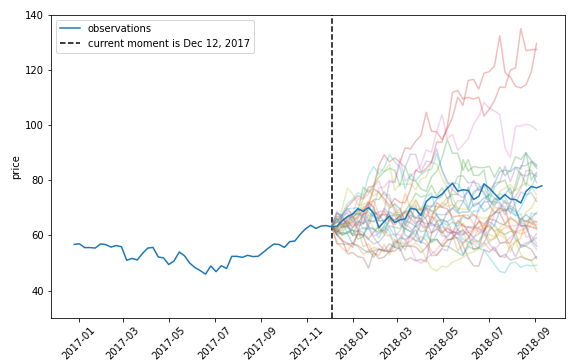
\includegraphics[width=0.6\textwidth]{potential_future.png}
    \caption{Brent crude oil prices for the period from December 26, 2016 to September 10, 2018 and potential future changes starting from December 12, 2017.}
    \label{fig:potential_future}
\end{figure}

In a rapidly changing environment, probabilistic forecasts are becoming increasingly important as they help to understand an uncertanty and underlying risks. For example, selection of target quantiles based on historical sales and stock-out costs of products makes forecasts useful for inventary planning. The fact that sales of modern smartphones can have significant peaks can require a quantile as high as 0.9 to protect againts the risk of the lack of stock. Probabilistic forecast are used in any situations where robust decisions should be made against uncertanty, such as budgeting decisions, trading and hedging strategies. For example, commodity trading companies can decide to optimize a portfolio to reduce risks if a range of supposed losses/profit is too wide. Novel risks involved by COVID-19 pandemic and climate changes clearly show that uncertanty assessment play a key role in the decision making. Another rationale for probabilistic forecasting is that it can determine how much to trust the predictions for underlying problems, as well as distinguish between regions with high and low uncertanty. For example, seasonal sales can be accurately forecasted for periods with high demand, while other periods can have wide range of possible sales.

In many cases, one-dimensional time series are statistically dependent on each other, and this dependency can also be taken into account to improve the accuracy of forecasts \cite{normflow2021}. For example, forecasting total sales of two negatively correlated products involves the fact that simultaneously increasing sales of both products is unrealistic, while independent forecasts cannot account this property. Examples of such behavior are depicted in the figure \ref{fig:correlation_ts}. The effect of interacting items is known as the cannibalization effect and it is of great importance in the retail business. In addition, in dealing with economic variables, the value is often not only related to its historical movements, but also to historical movements of other variables. For example, interest rate, income, and investment expenditures may have a large impact on the forecasting household consumption expenditures. Thus, it makes sense to use all available variables using a multivariate forecast instead of an individual ones.

\begin{figure}[!ht]
    \centering
    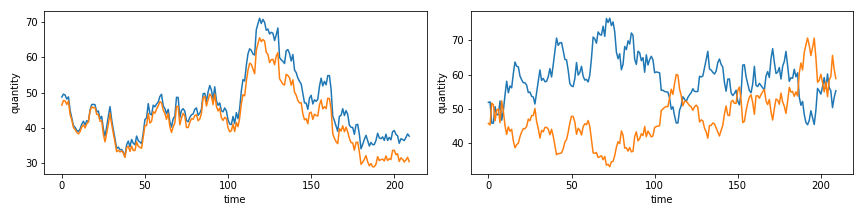
\includegraphics[width=0.99\textwidth]{correlation_ts.png}
    \caption{Generated time series. On the left are highly correlated time series, the correlation is 0.98. On the right are highly negatively correlated time series, the correlation is -0.98. }
    \label{fig:correlation_ts}
\end{figure}

Despite the fact that classical statistical methods of time series forecasting are often used by forecasting practitioners \cite{rnn2019}, recently more and more scientific papers on the use of neural networks for time series forecasting have appeared. Most of them are based on recurrent neural networks, attention-based models, and temporal convolutional networks \cite{tsdeeplearning2021}. In addition, recent public competitions in time series forecasting, such as M4 in 2018 \cite{MAKRIDAKIS202054} and M5 in 2020 \cite{m52020}, have shown that the best quality is achieved by gradient boosting models and neural networks \cite{m52020}. Previously, the use of neural networks was complicated by the fact that they are much more complex than classical statistical models and therefore require more historical data for training, in addition, they require specialists to understand the work and tuning of neural networks. However, now we live in the era of Big Data, companies collect a huge amount of data from day to day, which contains important information about the patterns of their business. In conditions where high-precision forecasting requires the use of all available information, complex models such as neural networks gain a great advantage.

Neural networks have already become popular in many data analysis tasks related to image, video, audio, and text processing. In addition, generative models of neural networks (deep generative models) are actively used in such tasks \cite{introductiondgm2021}. A distinctive feature of such models is that they are able to generate new observations based on previously seen ones. For example, generative adversarial networks (GANs) proposed in \cite{goodfellow2014} are actively used to generate new images \cite{choi2018stargan} and sound \cite{oord2016wavenet}. However, the use of such models for generating time series is only beginning to develop. Generative models can be used not only for generating time series and then obtaining a probabilistic forecast \cite{koochali2020like}, but also for backtesting and improvement the robustness of business strategies \cite{lezmi2020improving}. For example, to check the quality of a trading strategy, the time series is divided into two periods: "in-sample" (train period) and "out-of-sample" (test period). The purpose of this separation is to use the best parameters found on the "in-sample" period and then test the quality of such a strategy on the "out-of-sample" period. This approach has two drawbacks. First, it reduces the number of observations available for training the model, in addition to removing the most relevant observations from the train period, which may contain important information about the trend, seasonality changes and so on. Secondly, it is still based on only one validation split, since we observe only one realization of an unknown random process. To partially solve the second drawback in \cite{fpp3}, a cross-validation method for time series was proposed, which is based on the sequential division of the time series into pairs of periods "in-sample" and "out-of-sample". Generative models offer a new approach to solving this problem — to generate a time series whose characteristics will correspond to the real time series and then get a set of pairs of periods "in-sample" and "out-of-sample". The peculiarity of deep generative models is that they are able to take into account the characteristics of real financial time series: nonlinear autocorrelations, heavy tails, heteroskedasticity, regime change, and non-stationary properties \cite{lezmi2020improving}. For example, the Quant GAN model, as shown in \cite{quantgan2020}, is able to model such characteristics of financial time series.

Several deep generative models for time series forecasting have been proposed in recent years. All of them showed excellent quality and superiority over their competitors. At the same time, different models were considered as the baselines, different datasets, and different quality metrics were used in these works. Some of the models were tested on univariate forecasting, while others were tested on multivariate forecasting. The objectives of this work are:
\begin{itemize}
    \item Comparison of such models with each other on the same dataset and quality metrics.
    \item Presentation of the taxonomy of such models and possible directions for their development and modifications.
\end{itemize}

\section{Background}

\subsection{Probabilistic modeling}

We start from the point (deterministic) forecasting model. Let $y_t \in \mathbb R$ be a single value at the time moment $t$ and $y_1, y_2, \dots, y_T$ be known historical values. Then the $h$-step-ahead forecasting model can be defined as 
$$\hat{y}_{T+h} = f(y_T, y_{T-1}, \dots)$$
where $h$ is a predictable horizon. For example, $h=1$ for daily time series data means forecasting tomorrow's values. Multivariate forecasting model can be naturally generalized as
$$\hat{\mathbf y}_{T+h} = f(\mathbf y_T, \mathbf y_{T-1}, \dots)$$
where $\mathbf y \in \mathbb R^K$ and $i \in \{1, \dots, K\}$ is an identificator of an individual component of the time series \cite{mts2007}. For example, $y_{1,t}$ can represents sales of the item 1 and $y_{2,t}$ is sales of the item 2. 

Generalizing the deterministic model, we can introduce the probabilistic forecasting model. We denote the triple ($\Omega$, $\mathcal F$, $P$) as a probability space, where $\Omega$ is the set of elementary events, $\mathcal F$ is a sigma-algebra of these events, and $P$ is the probability measure defined on $\mathcal F$. The $K$-dimensional random vector $\mathbf y$ is a function defined on $\Omega$ such that for any real $K$-dimensional number $c$ there exists an event $A_c$ and
$$A_c = \{ \omega \in \Omega | y_1(w)\leq c_1, \dots, y_K(w) \leq c_K\} \in \mathcal F$$
Thus, the joint distribution function $F: \mathbb R^K \to[0, 1]$ is defined as $F(c)=P(A_c)$. Let us denote $p_\mathbf z$ as a set of indexes described a time axis, say positive integers $Z = \{1, 2, \dots\}$. Then we define a $K$-dimensional vector stochastic process as a function 
$$\mathbf y: Z \times \Omega \to \mathbb R^K$$
For any fixed $t \in Z$, the proccess $\mathbf y_t$ is a $K$-dimensional random vector. Thereby, the any fixed $\omega$ describes some realization of the stochastic process $\mathbf y_1(\omega), \mathbf y_2(\omega), \dots$. The underlying stochastic process is often called the data generating process, or generative model \cite{mts2007}.

In terms of probabilistic forecasting, we want to model a conditional joint distribution function of forecasted values with given historical observations
$$F_\mathbf{y}(\mathbf y_{T+h} | \mathbf y_{T}, \mathbf y_{T-1}, \dots)$$
and then calculate point forecasts or prediction intervals from this distribution. Often we work with absolutely continuous random vectors and then we model a joint probability density function
$$p_\mathbf{y}(\mathbf y_{T+h} | \mathbf y_{T}, \mathbf y_{T-1}, \dots) = \frac{\partial^K F_\mathbf{y}(\mathbf y_{T+h} | \mathbf y_{T}, \mathbf y_{T-1}, \dots)}{\partial y_{1, T+h}\dots\partial y_{K, T+h}}$$
Thereby, a point forecas can be obtained as the conditional expectation
$$\hat{\mathbf y}_{T+h} = \mathbb E[\mathbf y_{T+h} | \mathbf y_{T}, \mathbf y_{T-1}, \dots]$$
while, for example, the 0.95 quantile of $i$-th time series is obtained from a marginal cumulative distribution function as
$$\hat{y}_{i, T+h} = \{ y_{i, T+h} | F_\mathbf{y}(y_{i, T+h} | y_{i, T}, y_{i, T-1}, \dots) = 0.95 \}$$
Note the fact that marginalization makes the prediction intervals of the different components independent, and as a result, the forecast loses information about how realistic future movements of certain components will be.

\subsection{Vector autoregressive model}

The Vector Autoregressive (VAR) model is a classical statistical method for the multivariate forecasting \cite{mts2007} and it is the generalization of univariate autoregressive (AR) model. The VAR model of the order $p$ is denoted as VAR($p$) and it is defined via a system of linear equation
$$\mathbf y_{t} = \nu + A_1 \mathbf y_{t-1} + A_2 \mathbf y_{t-2} + \dots + A_p \mathbf y_{t-p} + \varepsilon_t$$
where $A_i$ are fixed ($K\times K$) coefficient matrices, $\nu$ is a fixed ($K \times 1$) intercept vector that is used in case of a non-zero mean of some individual time series, and $\varepsilon$ is a $K$-dimensional white noise or innovation process that holds the properties $\mathbb E [\varepsilon_t] = 0$, $\mathbb E [\varepsilon_t \varepsilon_t^\top] = \Sigma_\varepsilon$ and $\mathbb E [\varepsilon_t \varepsilon_s^\top] = 0$ for any $t\neq s$. Note that the noise vector is distributed as $\mathcal N(0, \Sigma_\varepsilon)$ and can be correlated among individual series, but $\varepsilon_t$ and $\varepsilon_s$ are independent if $t \neq s$.

The forecasting via VAR model is performed in a recursive manner. $p$ historical vectors $\mathbf y_{t-1}, \dots, \mathbf y_{t-p}$ are fed into VAR model and probabilistic forecasting of individual time series is calculated as
$$y_{i, t} \sim \mathcal N([\nu + A_1 \mathbf y_{t-1} + A_2 \mathbf y_{t-2} + \dots + A_p \mathbf y_{t-p}]_i, [\Sigma_\varepsilon]_{i,i})$$
where $[\cdot]_i$ is an i-th element of the vector and $[\cdot]_{i,i}$ is the element on an i-th row and i-th column of the matrix. For example, if $[\nu + A_1 \mathbf y_{t-1} + A_2 \mathbf y_{t-2} + \dots + A_p \mathbf y_{t-p}]_i = m$ and $[\Sigma_\varepsilon]_{i,i} = \sigma^2$ then the 95\% prediction interval be $m \pm 1.96 \sigma$. Next, the expected  vector $\hat {\mathbf y}_t = \mathbb E [\mathbf y_t]$ are fed into VAR model to obtain probabilistic forecast for $\mathbf y_{t+1}$.

The fitting of the parameters $\nu, A_1, \dots, A_p, \Sigma_\varepsilon$ can be performed by maximum likelihood (ML) estimation or least sqares (LS) estimation \cite{mts2007}.

The selection of the hyperparameter $p$ is performed by minimizing the Bayesian Information Criterion (BIC) that defined as
$$\text{BIC} = m \ln (n) + 2 \ln (\hat L)$$
where $m$ is the number of parameters estimated by the model that equivalent to $pK^2 + K$ in case of the VAR($p$) model, $n$ is the number of observations and $\hat L$ is the likelohood of the model.

\subsubsection{Transformations for stationarity}

There are three assumptions under the VAR model. First, we assume that the stochastic process is stationary, that is $\mathbb E (\mathbf y_t) = \mu$ for all $t$ and $\mathbb E [(\mathbf y_t - \mu)(\mathbf y_{t-h}-\mu)^\top] = \Gamma(h) = \Gamma(-h)^\top$ for all $t$ and $h$. Second, the determenistic part of components of stochastic proccess linearly depend on each other. Third, the errors of forecasts are described by the white noise.

The most time series are non-stationary in practice, but they can be transformed into stationary using the differencing operator in some cases
$$\Delta^d y_t = (1 - L)^d y_t$$
where $L$ is the lag operator $Ly_t = y_{t-1}$. The time series that can be transformed into stationary by $d$-differencing is called integrated of order $d$. The more times the difference operator is applied, the less accurate the predictions will be. The seasonal differencing operator $L^my_t = y_{t-m}$ can be useful, because it helps to make a time series stationary by using the differentiation operator less times in highly seasonal time series. To check that the time series is stationary is performed unit root tests, for example Kwiatkowski-Phillips-Schmidt-Shin (KPSS) test \cite{fpp3}. To stabilize the variance, there is common practice to use Box-Cox transformation
$$y_t^* = \begin{cases}
    \ln y_t & \text{if $\lambda = 0$} \\ 
    \frac{y_t^\lambda - 1}{\lambda} & \text{otherwise}
\end{cases}$$
where the parameter $\lambda \in \mathbb R$ can be selected by Guerro estimation \cite{guerrero93}.

\subsection{Deep generative models} \label{deepgenmodels}

The main goal of generative modeling is to obtain a representation of the intractable distribution $p_\mathbf y$ defined on $\mathbb R^K$. As a rule, $K$ is quite large and the distribution is quite complex. As a training set, we have independent identically distributed observations from the distribution $p_\mathbf y$. Our goal is to find a generator that can map observations from a simple prior distribution $p_\mathbf z$ defined on $\mathbb R^q$ to the distribution $p_\mathbf y$
$$G: \mathbb R^q \to \mathbb R^K$$
In other words, the generator translates samples (random noise) from a simple distribution $\mathbf z \sim p_Z$ to a distribution $\mathbf y \sim p_\mathbf y$ such that $G(\mathbf z) \approx \mathbf y$. As a common practice, $K$ i.i.d. Gaussian random variables $\mathcal N(0, 1)$ are selected as the prior distribution, that is $p_{\mathbf z} = \mathcal N(0, I_K)$.

In terms of the time series forecasting, we want to model the conditional distribution $p_\mathbf y(\mathbf y_{T+h} | \mathbf y_{T}, \mathbf y_{T-1}, \dots)$ and it can be approximated as
\begin{equation}\label{eq:gen}
\begin{aligned}
p_\mathbf y(\mathbf y_{T+h} | \mathbf y_{T}, \mathbf y_{T-1}, \dots) &= \int p_\mathbf y(\mathbf y_{T+h}, \mathbf z| \mathbf y_{T}, \mathbf y_{T-1}, \dots)\mathrm{d}\mathbf z\\ 
&= \int p_\mathbf y(\mathbf y_{T+h} | \mathbf z, \mathbf y_{T}, \mathbf y_{T-1}, \dots)p(\mathbf z) \mathrm{d}\mathbf z\\ 
&= \mathbb E_\mathbf z[\mathbf y_{T+h} | \mathbf z, \mathbf y_{T}, \mathbf y_{T-1}, \dots]\\ 
&\approx G(\mathbf z, \mathbf y_{T}, \mathbf y_{T-1}, \dots)        
\end{aligned}
\end{equation}
Thus, the generator should be able to model the conditional distribution with the given historical observations so that $G(\mathbf z, \mathbf y_{T}, \mathbf y_{T-1}, \dots) \approx \mathbf y_{T+h}$ where $\mathbf z \sim p_Z$ and $\mathbf y_{T+h} \sim p_\mathbf y$($\mathbf y_{T+h} | \mathbf y_{T}$, $\mathbf y_{T-1}$, $\dots$).

For many datasets with high dimensionality and complex dependencies between components, it is becoming common practice to use deep neural networks as universal approximators \cite{introductiondgm2021}. Such neural networks can be denoted as $G_\theta$, where $\theta$ means the trainable parameters of the neural network. The training of the generator is performed by updating trainable parameters $\theta$ by gradint descend with respect to the loss function $L_G$ that somehow measures the dissimilarity between the generated distribution and the observed one.

\subsubsection{Direct parametric approach}

One of the most simple methods of modeling a distribution of time series using neural networks is to train the parameters of some predetermined distribution \cite{tsdeeplearning2021}. For example, the multivariate Gaussian distribution is often used so that
$$\mathbf y_{T+h} \sim \mathcal N(\mu(\mathbf y_{T}, \mathbf y_{T-1}, \dots), \Sigma(\mathbf y_{T}, \mathbf y_{T-1}, \dots))$$
where $\mu$ and $\Sigma$ are outputs of a neural network. The mean vector $\mu$ has a dimension of $K \times 1$ while the covariance matrix $\Sigma$ has a dimension of $K \times K$, so the number of estimated parameters increases quadratically with the growth of the time series components, which makes learning very difficult. To solve this problem, a diagonal covariance matrix is used, $\Sigma_{ij} = 0$ for all $i \neq j$. In this case, the matrix is described only by diagonal elements that represented by a single vector $K \times 1$. Thus, the output of the network is $2K$-dimensional. To ensure that the standard deviations take only positive values, we can add softplus function before the network outputs $\Sigma$.

Fitting the network parameters is performed by the maximum likelihood estimation (or that equivalent, minimization of the negative log-likelihood). For example, for the multivariate Gaussian distribution with diagonal covariance matrix, we can consider components as independent variables and then for any individual target $p_\mathbf y$, we have a pair of mean $\mu_i$ and standard deviation $\sigma_i$. In this case, the negitive log-likelihood is calculated as
$$\begin{aligned}
L_{G} &=-\ln \ell(\mu, \sigma \mid y) \\
&=-\ln \left(\left(2 \pi \sigma^{2}\right)^{-1 / 2} \exp \left[-(y-\mu)^{2} /\left(2 \sigma^{2}\right)\right]\right) \\
&=\frac{1}{2} \ln (2 \pi)+\ln (\sigma)+\frac{(y-\mu)^{2}}{2 \sigma^{2}}
\end{aligned}$$

In this limit case, the generator is the identity function $G(\mathbf z, \mathbf y_{T}, \mathbf y_{T-1}, \dots) = \mathbf z$, because the forecasts are already described by tractable simple distribution. We can easily generate future observations from the multivariate Gaussian distribution to obtain a probabilistic forecast.

\subsubsection{Generative adversarial network}\label{gan}

Generative adversarial networks (GANs) are a distribution modeling strategy that uses two neural networks: the generator $G$ and the discriminator $D$. The generator $G$ performs the task of translating samples from a relatively simple distribution of $p_\mathbf z$ to a rich, complex, multivariate distribution of a stochastic process $p_\mathbf y$. The task of discriminator $D$ is to distinguish the true data from the generated data. The generated and true data in the GAN context are called fake and real data. Strictly speaking, the discriminator's task is to minimize the binary classification error from input data that contains both real and fake data. On the other hand, the task of the generator is to generate such fake data so that it is as difficult as possible for the discriminator to distinguish them from the real ones. The generator and discriminator are trained simultaneously, so they compete until the generator is able to generate indistinguishable data from the real data.

From the mathematical point of view, a generator is a function that translates vectors of one space into a vector of another space $G: \mathbb R^q \to \mathbb R^K$, as described in the section \ref{deepgenmodels}. Let say that the generator model the distribution $p_\mathbf{\hat y}$ that we want to as close as possible to the real distribution $p_\mathbf y$. The discriminator is a function that evaluates how likely the observation is to be real, $D: \mathbb R^K \to [0, 1]$, where 0 means fake data and 1 means real data. Thus, 0.5 means that for the discriminator, such data looks equally real and fake. As previously mentioned, the generator and discriminator are trained simultaneously, that is, they play a two-player minimax game with the value function $V$
$$\begin{aligned}
\min _{G} \max _{D} V(D, G) =\mathbb{E}_\mathbf{y}[\ln D(\mathbf{y})]+ \mathbb{E}_\mathbf{z}[\ln (1-D(G(\mathbf{z})))]
\end{aligned}$$
The training of the generator and discriminator takes place in steps, so the value function is decomposed into two functions: discriminator's loss function 
$$L_D = -\mathbb{E}_\mathbf{y}[\ln D(\mathbf{y})] - \mathbb{E}_{\mathbf{z}}[\ln (1-D(G(\mathbf{z})))]$$
and generator's loss function
$$L_G = -\mathbb{E}_{\mathbf{z}}[\ln (D(G(\mathbf{z})))]$$
according to which the weights of the neural networks are updated step-by-step. As a rule, $l>1$ steps of the discriminator optimization are performed, and then the single step of the generator optimization is made.  As was shown in \cite{goodfellow2014}, the value function with the optimal discriminator $D^*$ is 
$$V(D^*, G)=-\ln (4)+2 \cdot \text{JSD}(p_\mathbf{y} \| p_\mathbf{\hat y} )$$
where JSD is the Jensen–Shannon divergence between the model’s distribution and the data generating process. Thus, the generator learns to minimize the JSD and then in the case of identical distributions $p_\mathbf{y}$ and $p_\mathbf{\hat y}$, the value function be in the global optimum $V^* = - \ln (4)$.

GANs for probabilistic forecasting has been proposed in \cite{koshiyama2019generative} and \cite{koochali2020like}. Here we want to model the conditional distribution $p_\mathbf y(\mathbf y_{T+h}|\mathbf{y}_{T}, \mathbf{y}_{T-1}, \dots)$ via the generator $G$($\mathbf z$, $\mathbf{y}_{T}$, $\mathbf{y}_{T-1}$, $\dots$), and then the discriminator should classify the sequence $\mathbf y_{T+h}, \mathbf{y}_{T}, \mathbf{y}_{T-1}, \dots$, where $\mathbf{y}_{T}, \mathbf{y}_{T-1}, \dots$ are historical observations, and $\mathbf y_{T+h}$ is real or fake. Thereby, the full conditional value function $V$ is 
$$
\begin{aligned}
\min _{G} \max _{D} V(D, G) =\mathbb{E}_\mathbf{y}[\ln D(\mathbf y_{T+h} | \mathbf{y}_{T}, \mathbf{y}_{T-1}, \dots)]\\
+ \mathbb{E}_\mathbf{z}[\ln (1-D(G(\mathbf z | \mathbf{y}_{T}, \mathbf{y}_{T-1}, \dots) | \mathbf{y}_{T}, \mathbf{y}_{T-1}, \dots))]    
\end{aligned}
$$
where $G(\mathbf z | \mathbf{y}_{T}, \mathbf{y}_{T-1}, \dots)$ is a probabilistic form of the generator \eqref{eq:gen} in the sence that $\mathbf z$ is the random variable, but not a sample from the prior distribution.

One of the problems in GAN training is that there are no convergence guarantee. Two models are trained simultaneously to find a Nash equilibrium in a non-cooperative two-player game. However, each model updates its parameters independently of the other player in the game. Simultaneous updating of the gradient of both models cannot guarantee convergence. As we can see in the figure \ref{fig:gan}, the loss functions fluctuate, and there is no observed convergence.

\begin{figure}[!ht]
    \centering
    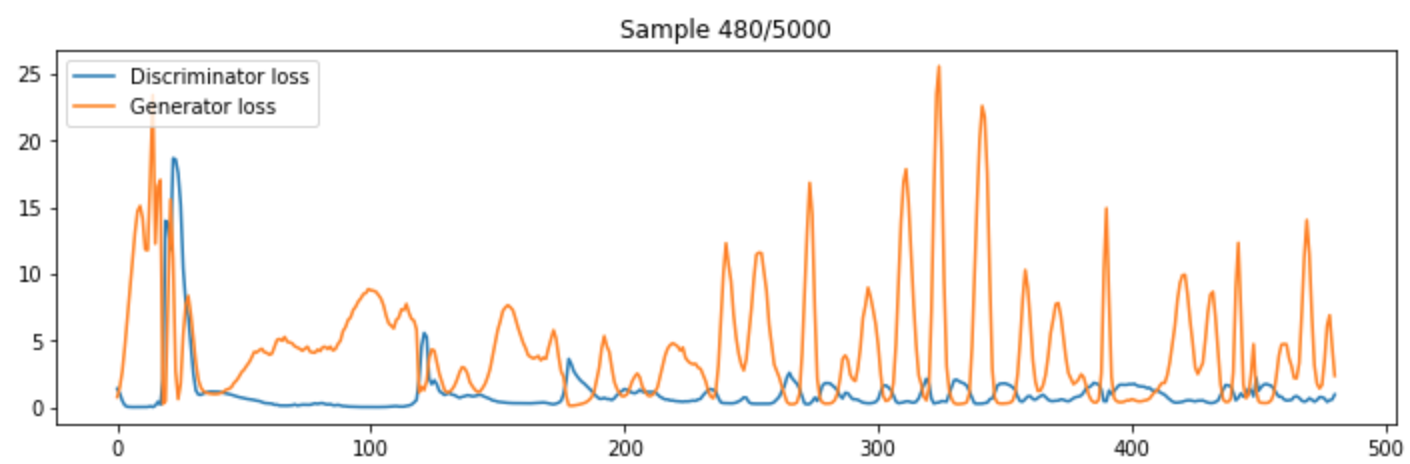
\includegraphics[width=0.8\textwidth]{gan.png}
    \caption{Loss functions during training GAN}
    \label{fig:gan}
\end{figure}

\subsubsection{Normalizing flow}

The Normalizing flow \cite{normflow2021} is the generator of the form $G: \mathbb R^q \to \mathbb R^K$ where $q=K$ and consists of a sequence of invertible functions. Each function $f$ makes the transformation of initial density function as follows
$$p_{\mathbf{y}}(\mathbf{y})=p_{\mathbf{z}}(\mathbf{z})\left|\operatorname{det}\left(\frac{\partial f(\mathbf{y})}{\partial \mathbf{y}}\right)\right|$$
where $\partial f(\mathbf y)/\partial \mathbf y$ is the Jacobian of $f$ at $\mathbf y$. The main property of normalizing flows is they are designed so that the computing the Jacobian determinant takes no more than  $O(K)$ time and makes it easy to invert $f^{-1}(\mathbf z) = \mathbf y$.

There are a few options to define such functions. For example, Real NVP \cite{normflow2021} model is constructed on coupling layers that keep some inputs unchanged and transforms other inputs with respect to unchanged ones
$$
\begin{cases}
    \mathbf w^{1:k} = \mathbf y^{1:k} \\
    \mathbf w^{k+1:K} = \mathbf y^{k+1:K} \odot \exp(s(\mathbf y^{1:k})) + t(\mathbf y^{1:k})
\end{cases}
$$
where a superscript is the index of an input vector, $\odot$ is the Hadamard product, $s$ is a scaling, $t$ is a translation that are neural networks that map $\mathbb R^k \to \mathbb R^{K-k}$. To model the target distribution, $M$ coupling layers are connected together so that $\mathbf{y} \to \mathbf{w}_1 \to \mathbf{w}_2 \to \dots \to \mathbf{w}_{M-1} \to \mathbf{z}$. Using transormation density formula, the log likelihood of the target distribution can be written as
$$\log p_{\mathbf{y}}(\mathbf{y})=\log p_{\mathbf{z}}(\mathbf{z})+\log |\operatorname{det}(\partial \mathbf{z} / \partial \mathbf{y})|=\log p_{\mathbf{z}}(\mathbf{z})+\sum_{i=1}^{M} \log \left|\operatorname{det}\left(\partial \mathbf{w}_{i} / \partial \mathbf{w}_{i-1}\right)\right|$$
The log determinant of the Jacobian is calculated very simply, given that the Jacobian itself in this case has a block-triangular shape 
$$\log \left|\operatorname{det}\left(\partial \mathbf{w}_{i} / \partial \mathbf{w}_{i-1}\right)\right| = \log \left| \exp \left(\operatorname{sum}\left(s_{i}\left(\mathbf{w}_{i-1}^{1: d}\right)\right) \right) \right|$$
where $\operatorname{sum}$ is overall summation \cite{normflow2021}. Using such log-likelihood function we can define the generator's loss as
$$L_G = -\log p_\mathbf{y}(\mathbf y)$$
For probabilistic forecasting, the conditioning $p_\mathbf{y}(\mathbf{y}_{T+h}| \mathbf{y}_T, \mathbf y_{T-1}, \dots)$ can be performed via concatenation in every coupling layer $s(\operatorname{concat}(\mathbf w_i^{1:k}, \mathbf h_T))$ and $t(\operatorname{concat}(\mathbf w_i^{1:k}, \mathbf h_T))$ where $\mathbf{h}_T$ is some embedding of the historical observations $\mathbf y_{T}, \mathbf y_{T-1}, \dots$ that can be obtained from another neural network such as RNNs or self-attentions \cite{normflow2021}.

\subsection{Architectures for time series forecasting}

A neural network consists of interconnected layers that consist of neurons. Each neural network has an "input", "output" and some "hidden" layers. The number of neurons on the input layer determines the number of input variables. The number of neurons on the output layer determines the dimension of the output value. For example, to solve the regression problem $y = f (x_1, x_2, x_3)$, a neural network will need three input neurons and one output. Each layer has a set of trainable parameters that are updated during the training of the neural network. 

The simplest neural layer is the linear layer that has a matrix of trainable parameters $W$ and an intercept $b$. The linear layer performs a matrix multiplication of the form $xW^\top + b$. After each linear layer, an activation function is added that allows the neural network to learn complex nonlinear dependencies between variables. An example of such an activation function would be $\text{ReLU} (x) = \max (0, x)$. A neural network that consists only of linear layers and activation functions between layers is called a multi-layer perceptron (MLP) or feed forward network. 

To train neural networks, the back propagation mechanism is used. The idea is that the training of a neural network takes place step by step. Each step consists of two stages. The first stage is forward: data from the training sample is fed to the input of the neural network, and the output value is compared with the correct answer and the value of the loss function (error) is calculated. For example, the loss function $\text{MSE} = (y - \hat y)^2$ where $y$ is correct answer and $\hat y$ is an output of the network can be used for the regression task. The second backward stage is the calculation of the gradient of the loss function for performing gradient descent. Since the neural network can be quite complex and the calculation of the analytical solution is difficult, a step-by-step calculation of the gradient for each layer is performed, starting from the last one, which is then passed to the earlier layers using the chain rule
$$\frac{d y}{d x}=\frac{d y}{d u} \cdot \frac{d u}{d v} \cdot \frac{d v}{d x}$$
The training of the neural network is performed by updating trainable parameters $\theta$ by gradint descend so that
$$\theta \leftarrow \theta - \alpha \nabla_\theta L$$
where $\alpha$ is the learning rate and $L$ is the network's loss function.

Different combinations of layers give different neural network architectures. Some of these architectures are popular in time series forecasting problems, but these architectures themselves are only applicable in point forecasting. To get a probabilistic forecast, we need to use some kind of generative model. The exception is quantile regression models, which is essentially a set of point forecasts, but since a set of quantiles cannot define a joint distribution, such models are not considered in this work. Note that the generative models described earlier can be built on different architectures, so any combination of "generative model" + "architecture" determines a separate option for obtaining a probabilistic forecast.

\subsubsection{Neural network autoregression}

Neural network autoregression (NNAR) was described in \cite{fpp3}. Such a neural network is a feed forward network with a single hidden layer. The $\text{NNAR}(p,P,k)_m$ model is defined by 4 parameters, where $p$ is the number of previous observations to be input, $P$ is the number of seasonal observations, $k$ is the number of neurons on the hidden layer, and $m$ is the step for taking seasonal observations. Thereby, the full input of the network is ($y_{t-1}$, $y_{t-2}$, $\dots$, $y_{t-p}$, $y_{t-m}$, $y_{t-2m}$, $\dots$, $y_{t-Pm}$). For example, for the $\text{NNAR}(3, 2, 2)_{12}$ model, previous observations $y_{t-1}, y_{t-2}, y_{t-3}$, seasonal previous observations $y_{t-12}, y_{t-24}$ will be fed in the input, and a hidden linear layer with two neurons will be used for the model (it is shown in the figure \ref{fig:nnar}). By default, the output of the neural network is the forecasted next value $y_t$, so for forecasting the series at step $t+h$, it is performed according to the usual autoregressive manner — the previously forecasted value is fed in input. However, probabilistic forecasting requires a more flexible architecture in which we can use as many outputs as we need to implement the desired model. Therefore, for example, to implement the GAN model, we can use two NNAR neural networks, in which the generator will have the same number of outputs as the number of discriminator inputs.

\begin{figure}[!ht]
    \centering
    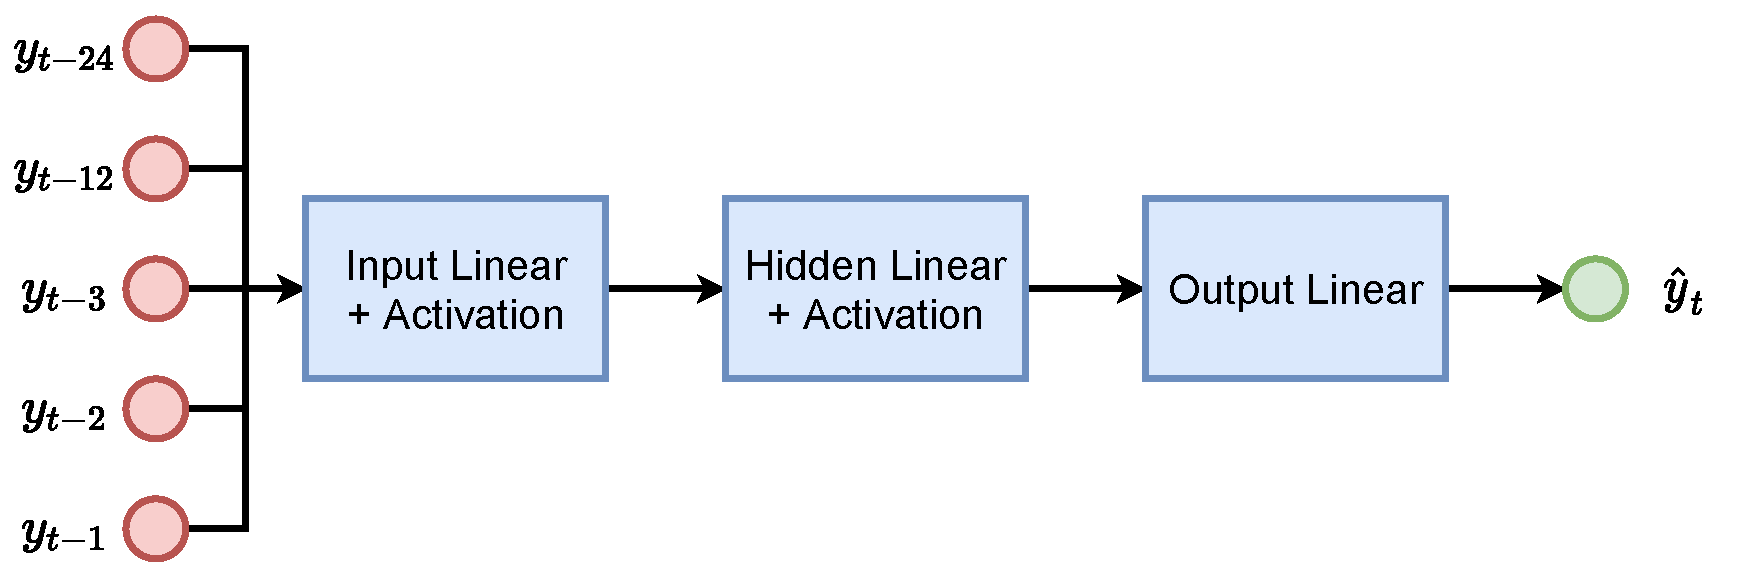
\includegraphics[width=0.8\textwidth]{nnar.pdf}
    \caption{An example of the $\text{NNAR}(p, P, k)_m$ model. The parameters are $p=3$, $P=2$, $k=2$, $m=12$. The predictable horizon $h=1$.}
    \label{fig:nnar}
\end{figure}

\subsubsection{Recurrent neural network}

Recurrent neural networks (RNNs) were proposed for sequence modeling, and they were especially popular in natural language processing (NLP) tasks. The sequence of words in a sentence is modeled by a time series, so time series forecasting has also become a natural use of such models. The main feature of such neural networks is that they have an internal memory that stores a compact representation of past observations. The internal memory is iteratively updated when new observations are received. RNN contains temporal block, each block in contains a few layers. For example, the Elman RNN block is defined as follows
$$
\begin{aligned}
    h_{t} &=\sigma_{h}\left(W_{h_1} x_{t}+W_{h_2} h_{t-1}+b_{h}\right) \\
    y_{t} &=\sigma_{y}\left(W_{y} h_{t}+b_{y}\right)
\end{aligned}
$$
where $h_t$ is a hidden state of the cell, $x_t$ is a input sequence, $y_t$ is the output sequence and $\sigma$ is an activation function. Since the model was originally developed for NLP problems, so there is an input and output sequence here. For example, for a machine translation task, $x_t$ can be a text in Russian, and $y_t$ can be a text in English. When forecasting time series, we work with a whole sequence, so to work with time series, we can use a special version of the modeling, in which $y_t = x_{t+1}$. A feature of recurrent neural networks is also that they do not require the selection of a certain number of previous observations, since the observations are processed sequentially one by one. An example of the RNN is depicted in the figure \ref{fig:lstm}. 

\begin{figure}[!ht]
    \centering
    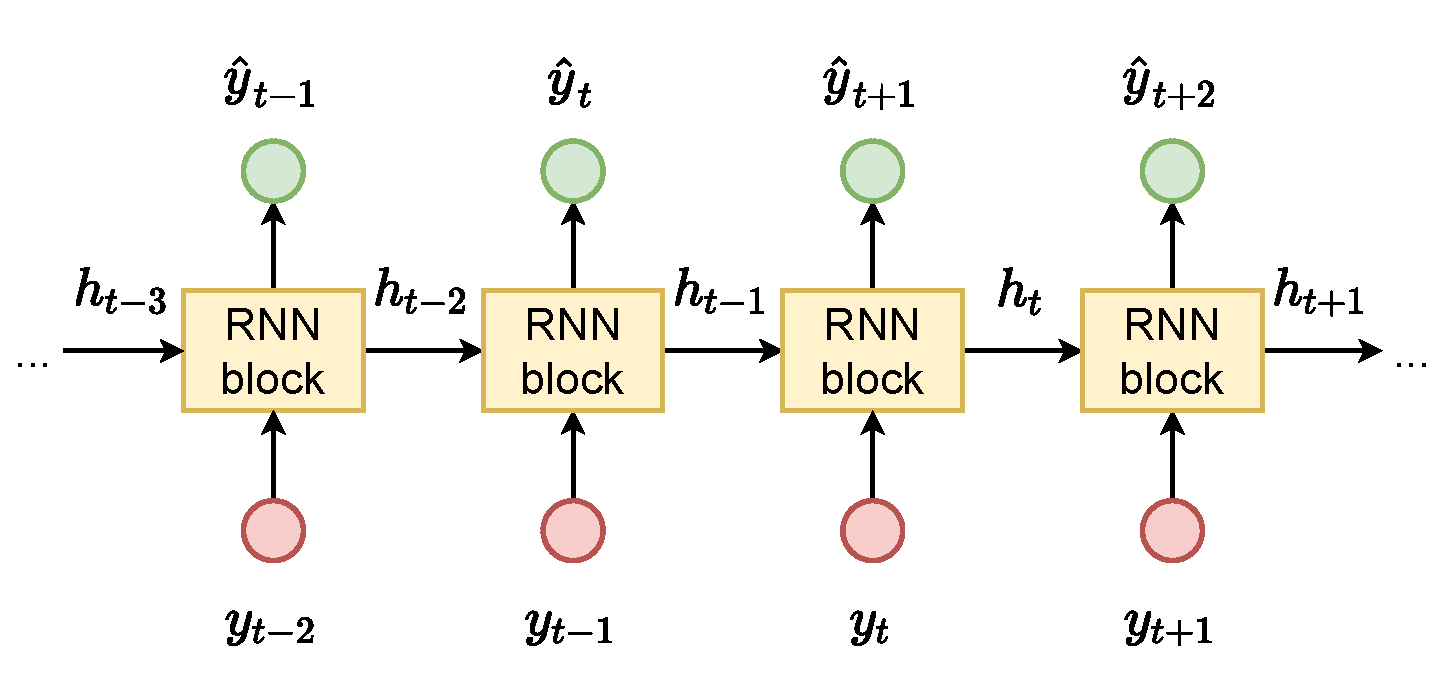
\includegraphics[width=0.8\textwidth]{lstm.pdf}
    \caption{An example of the RNN model. The predictable horizon $h=1$.}
    \label{fig:lstm}
\end{figure}

Due to some problems in the training (exploding and vanishing gradient) of Elman RNN, several other variants of recurrent networks were eventually developed. For example, the Long short-term memory (LSTM) model uses a special cell block state that stores long-term information transmitted through a sequence of observations. The LSTM block is defined via input gate, output gate, forget gate, hidden state and cell state as follows
$$
\begin{aligned}
\text { input gate: } {i}_{t} &=\sigma\left({W}_{i_{1}} {h}_{t-1}+{W}_{i_{2}} y_{t}+{b}_{i}\right) \\
\text { output gate: } {o}_{t} &=\sigma\left({W}_{o_{1}} {h}_{t-1}+{W}_{o_{2}} y_{t}+{b}_{o}\right) \\
\text { forget gate: } {f}_{t} &=\sigma\left({W}_{f_{1}} {h}_{t-1}+{W}_{f_{2}} y_{t}+{b}_{f}\right)
\end{aligned}
$$
and the states are
$$
\begin{aligned}
\text { hidden state: } h_{t} &=o_{t} \odot \tanh \left(c_{t}\right) \\
\text { cell state: } c_{t} &=f_{t} \odot c_{t-1}+i_{t} \odot \tanh \left(W_{c_{1}} h_{t-1}+W_{c_{2}} y_{t}+b_{c}\right)
\end{aligned}
$$
where $\tanh(\cdot)$ is the tanh activation fucntion. We can obtain the next observation $y_{t+1}$ using a linear layer so that
$$y_{t+1} = W_y h_{t} + b_y$$

\subsubsection{Attention-based model}

The attention mechanism has been proposed to improve long-term dependency learning \cite{bahdanau2016neural}. The transformer model was based entirely on the attention mechanism and achieved the best results in NLP tasks \cite{vaswani2017attention}. Recently, it was shown that the attention mechanism can improve perfomance of time series forecasts with respect to recurrent neural network \cite{tsdeeplearning2021}. The special feature of the attention mechanism is that it aggregates information using dynamic weights, allowing to literally "pay attention" to the right places in the sequence. One modification of the multi-head self-attention mechanism for time series forecasting was proposed in \cite{normflow2021}. The time series $Y = [\mathbf y_{T-t}, \dots, \mathbf y_{T-1}]^\top \in \mathbb R^{t \times K}$ are transformed into $h$ keys, queries and values that computed as
$$
\begin{aligned}
\text{keys: } K_i = Y W_i^K \\
\text{queries: } Q_i = Y W_i^Q \\
\text{values: } V_i = Y W_i^V \\
\end{aligned}
$$
where $W_i^Y \in \mathbb R^{K \times d_k}, W_i^Q \in \mathbb R^{K \times d_k}, W_i^V \in \mathbb R^{K \times d_v}$ are trainable matricies. The attention mechanism produces "heads" of the form
$$
\text{head}_i=\operatorname{Attention}\left(Q_i, K_i, V_i\right)=\operatorname{softmax}\left(\frac{Q_i K_i^{\top}}{\sqrt{d_{k}}} \cdot M\right) V_i
$$
where $M$ is a mask that can filter the rightward observations by defining all upper-triangular element as $-\infty$ so that we cannot pay attention to future time moments. Here the normalization by $d_k$ the dimension of the matricies is performed. The output of the attention layer is
$$O = \text {Concat}\left(\text{head}_{1}, \ldots, \text {head}_{h}\right) W^{O}$$
where $W^O \in \mathbb R^{hd_v \times d_\text{model}}$ and thereby $O \in \mathbb R^{t \times d_\text{model}}$. This mechanism is called multi-head scaled dot-product attention. The attension layer is used in encoder-decoder manner so that we can set $d_\text{model} = K$ to obtain the forecasted time-series in the same dimensionality as the input sequence. The example of the multi-head self-attention model is depicted in the figure \ref{fig:attention}.

\begin{figure}[!ht]
    \centering
    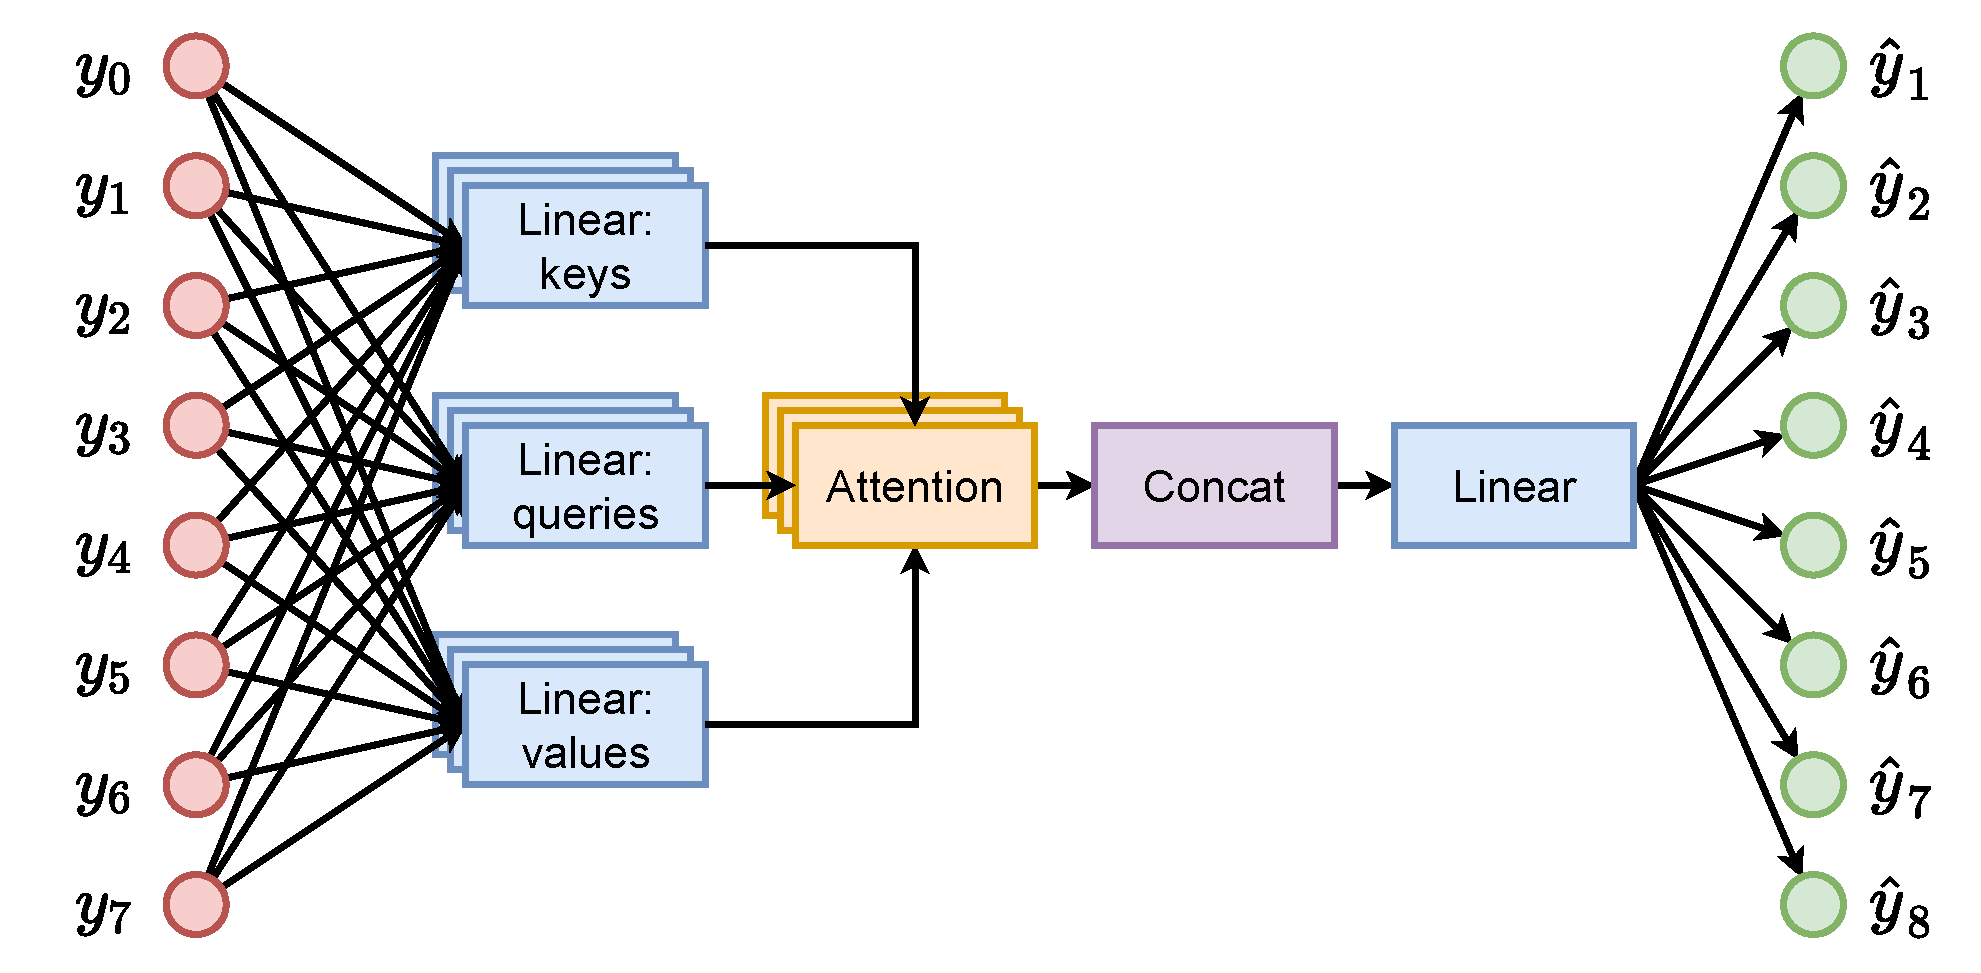
\includegraphics[width=0.8\textwidth]{attention.pdf}
    \caption{An example of the multi-head self-attention model. The predictable horizon $h=1$, the window size is 8.}
    \label{fig:attention}
\end{figure}

\subsubsection{Temporal convolutional network}

Temporal convolutional network (TCN) was proposed in \cite{BaiTCN2018} for sequence-to-sequence modeling
$$\hat{y}_{0}, \ldots, \hat{y}_{T}=f\left(x_{0}, \ldots, x_{T}\right)$$
but it can also be applied for time series forecasting by
$$\hat{y}_{0+h}, \ldots, \hat{y}_{T+h}=f\left({y}_{0}, \ldots, {y}_{T} \right)$$
The TCN is based on two principles: the network maps the original sequence into the sequence of the same length and there are no leakage from the future into the past. The first property is achieved by using one-dimensional full-convolution networks, where all hidden layers preserve the dimension of the input layer, and using zero-padding, which is added to preserve the length of the input sequence. To achieve the second property, the so-called causal convolutions is used, in which elements at time $t$ on the current layer cannot affect elements later than $t$ on the next layer. This is achieved by adding zero-padding only before the first value of each intermediate sequence.

Simple convolution has a disadvantage — the number of observations from the past that can be taken into account at the output of the neural network (receptive field) increases linearly with the growth of the network depth. To solve this problem, dilated convolution is used, which allows to increase the number of observations exponentially. Formally, dilated convolution is defined as follows
$$F(s)=\left(\mathbf{x} *_{d} f\right)(s)=\sum_{i=0}^{k-1} f(i) \cdot \mathbf{x}_{s-d \cdot i}$$
where $d$ is dilation factor, $k$ is the kernel size of the kernel $f: {0, 1, \dots, k-1} \to \mathbb R$. Thus, to increase the receptive field, we can use two approaches: increase the kernel, or increase the dilation factor. Typically, TCN uses an exponential growth dilation factor, such as $d = O(2^i)$ on the i-th layer. An example of dilated causal convolutions is presented in the figure \ref{fig:tcn}

\begin{figure}[!ht]
    \centering
    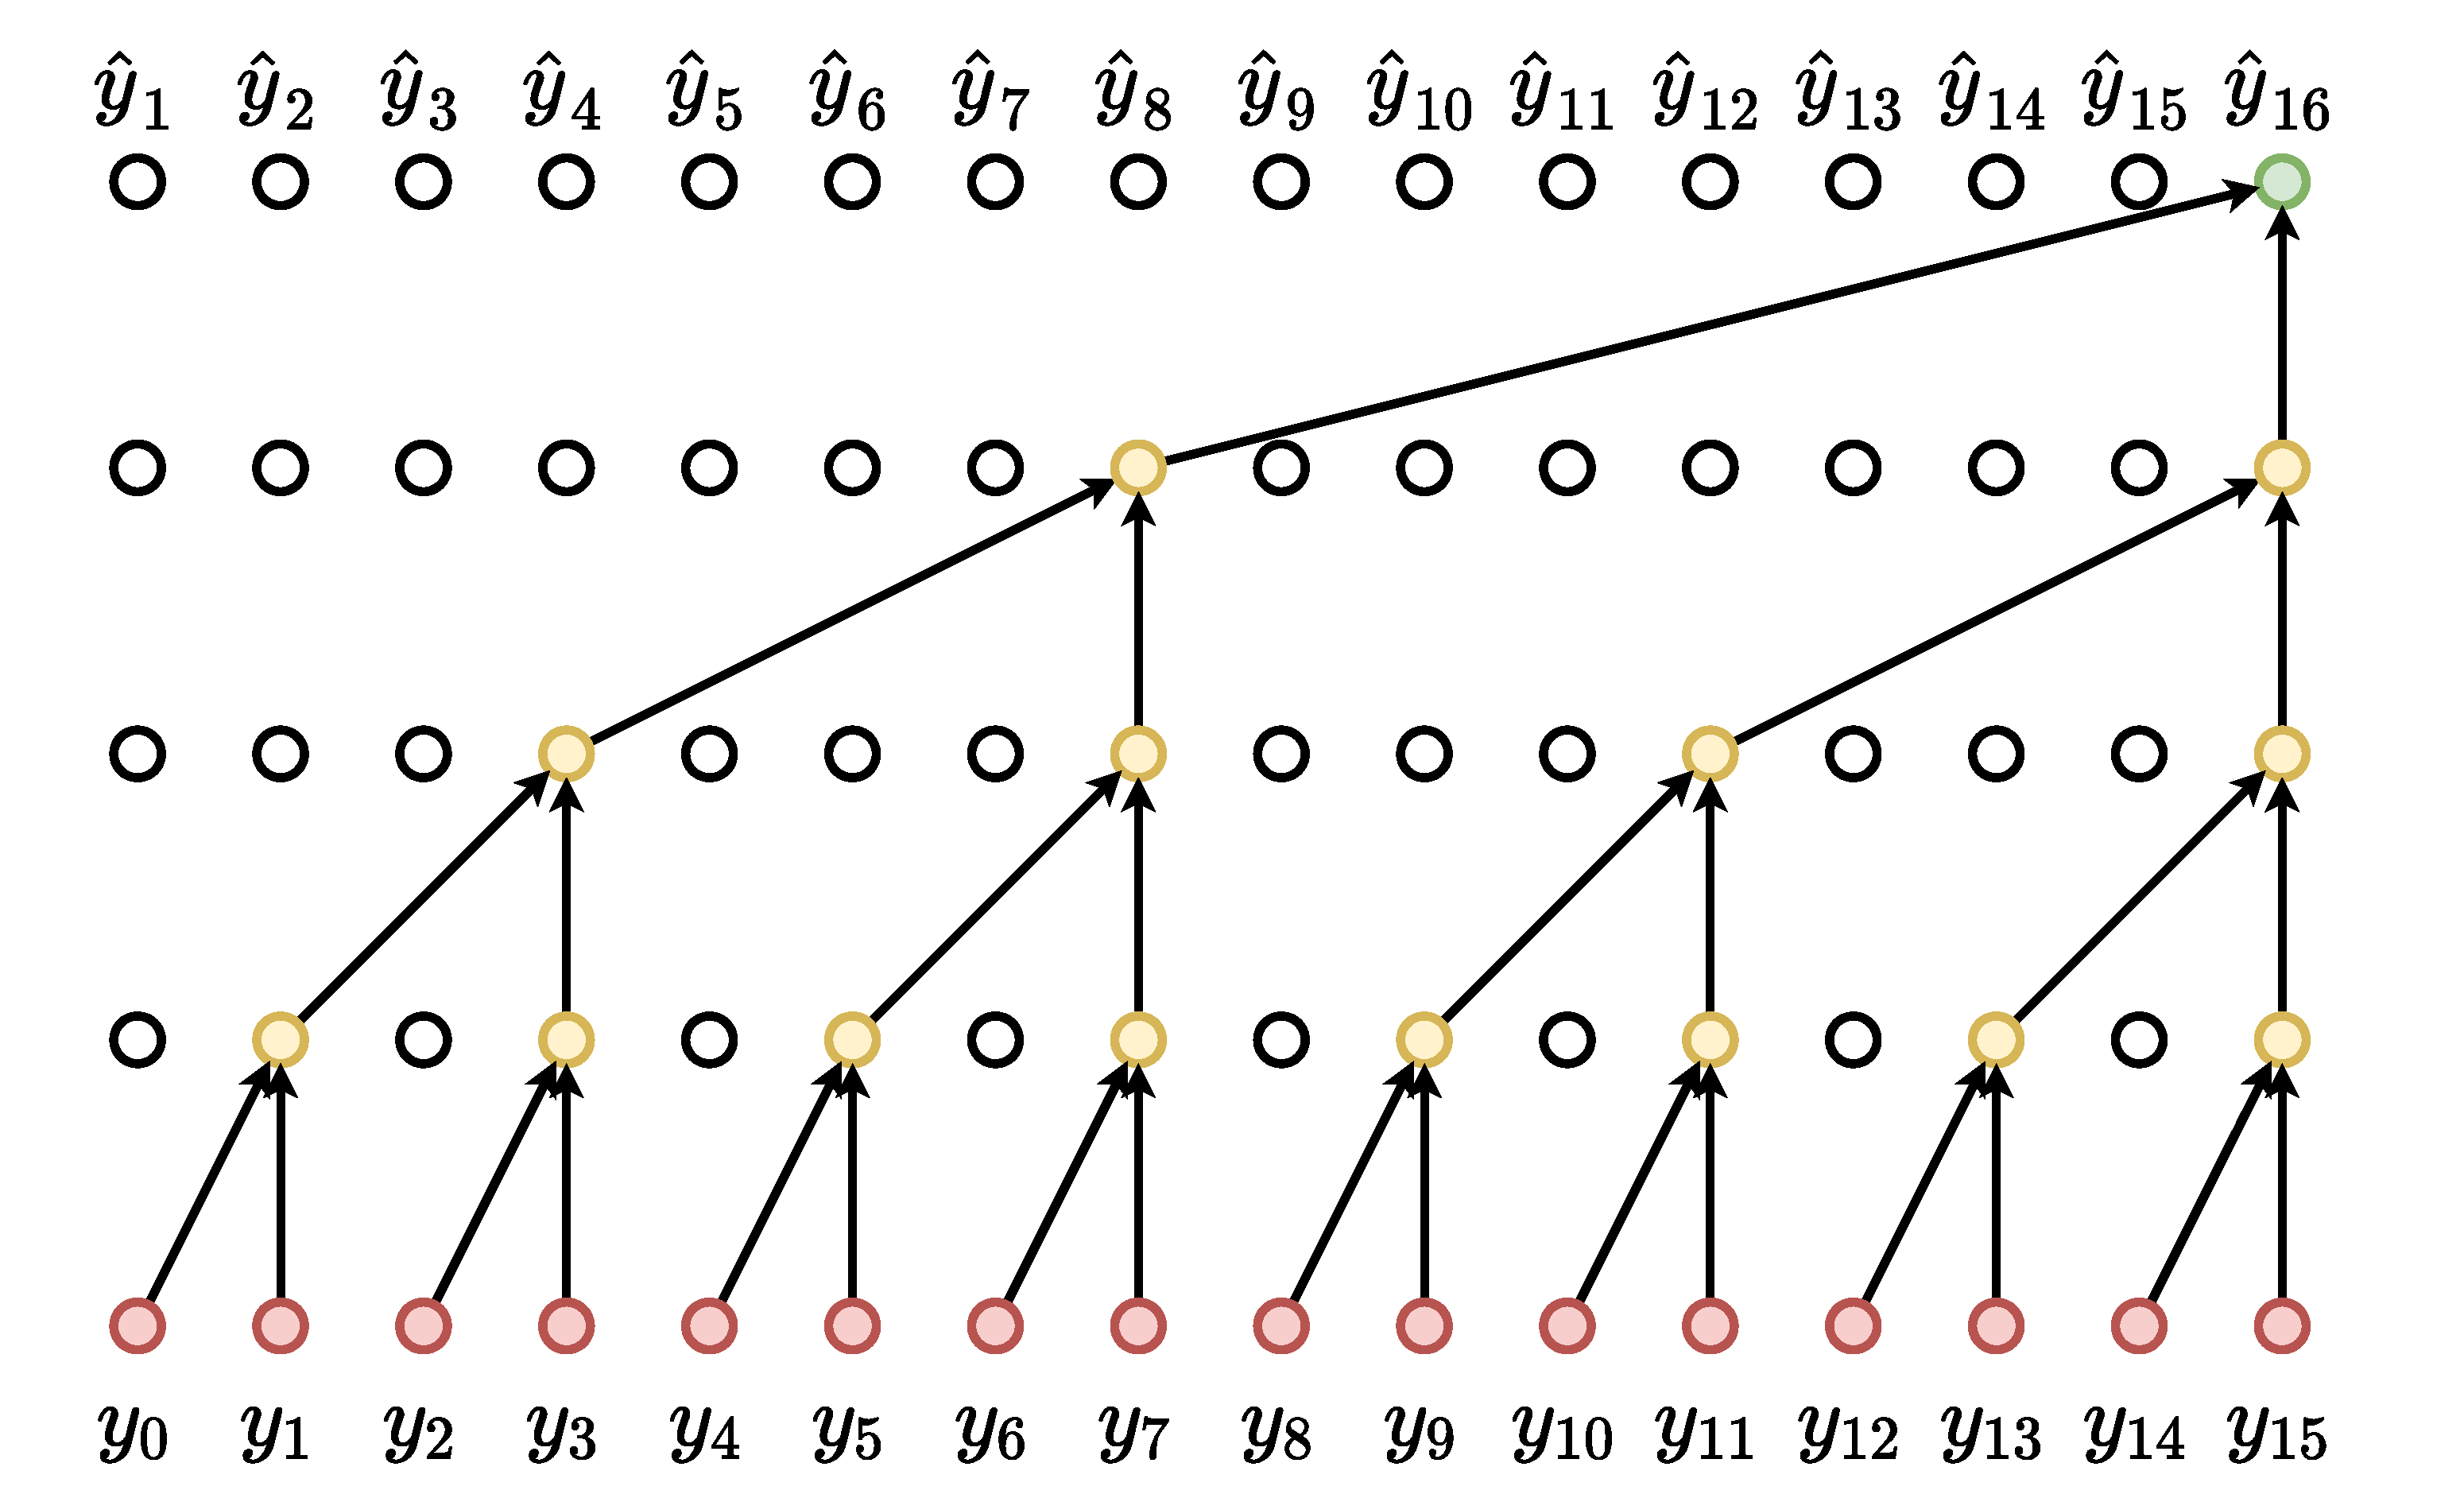
\includegraphics[width=0.8\textwidth]{tcn.pdf}
    \caption{An example of dilated causal convolutions. The number of convolutions is 4, dilation factor is $2^i$, kernel size is $2$. In this case, the receptive field will be 16. The predictable horizon $h=1$.}
    \label{fig:tcn}
\end{figure}

The TCN consists of several residual blocks that are connected in series. Each residual block consists of two causal convolutions and a residual connection so that the output of the blocks with respect to the input $\mathbf x$ is
$$o=\text {Activation}(\mathbf{x}+\mathcal{F}(\mathbf{x}))$$
where $\mathcal F$ is series of transformation $\text{Dilated causal convolution} \to \text{Weighted norm} \to \text{ReLU} \to \text{Dropout} \to \text{Dilated causal convolution} \to \text{Weighted norm} \to \text{ReLU} \to \text{Dropout}$.

\section{Literature reviews}

In the paper \cite{koochali2020like}, the probabilistic time series forecasting method ProbCast was presented. The idea of the method was that first the architecture of the model is selected, which makes a point forecast. It is assumed that the model has two linear layers at the output. After that, the input of the first linear layer is doubled, and the output of the previous layer is concatenated with the generated noise, thus creating a generative model. The authors have shown that this approach allows us to achieve an improvement in quality compared to the original point forecast model.

In \cite{normflow2021}, a model was proposed that uses a normalizing flow to generate time series, and to account for historical observations, the coupling layer combines information from the previous layer and from the hidden state of the module to obtain embeddings, such as LSTM or Transformer. The method showed the best values of the quality metric.

The papers \cite{quantgan2020} and \cite{tsgan} described models for generating time series using GAN. In the course of numerical experiments, it was shown that such models are able to take into account complex structures of time series behavior. In \cite{cganforts}, a TSGAN time series generation model was presented that uses two GAN models, i.e. 4 neural networks. The first GAN is used to generate spectrograms, which are then used as noise levels for the second GAN model. TSGAN has been shown to have the ability to generate realistic synthetic 1D signals across a multitude of data types: sensor, medical, simulated, motion, and other within human perceptual desire.

In the paper \cite{gaussiantcn2020}, examples of using TCN to obtain a probabilistic forecast using a direct probabilistic approach were given. In particular, options for obtaining a quantile forecast and the distribution parameters of a multivariate independent Gaussian distribution for a full probability forecast were presented. As a result of experiments, it was shown that the proposed method shows superiority in the quality and effectiveness of the forecast with other modern forecasting methods.

In \cite{deepar}, the DeepAR model based on the direct probability approach and RNN was proposed for the problem of forecasting one-dimensional time series. As a result of the tests, it was shown that this method shows the best efficiency compared to its competitors.

In the works \cite{multihorizon} and \cite{interpr}, a model was proposed that combines the Attention and RNN mechanism to obtain a probable forecast, which also showed the best quality among all the compared models.

The works \cite{BaiTCN2018} showed the effectiveness of using TCN for synthetic stress tests, polyphonic music modeling, character-level language modeling, and word-level language modeling, while \cite{borovykh2018conditional} proposed an effective conditional model for obtaining a point forecast using TCN.

\section{Experimental setup}

For testing, I chose several models that I found in recent papers on probabilistic forecasting. They use different approaches to generative modeling and are built on different architectures. The choice of models was based on the results of testing conducted by the authors of the articles, as well as on the availability of open source code or an exhaustive description of the algorithm. Note that these models contain some tricky implementation details, and they are not precisely implemented as mentioned earlier, just combining a generative approach and a network architecture, but contain its main components.

\textbf{VAR} is the classical statistical model \cite{fpp3}. Before passing into the model, each time series dataset was preprocessed by seasonal differencing and Box-Cox transformation to make it stationarity as close as possible. The stationarity was checked using the KPSS test. The order of the model was selected using the BIC criterion. The transformation, forecasting, inverse transformation pipeline is depicted in the figure \ref{fig:transformation_var}

\begin{figure}[!ht]
    \centering
    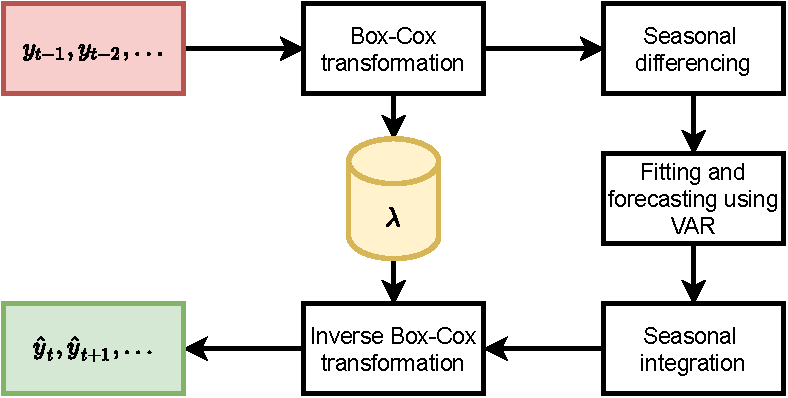
\includegraphics[width=0.6\textwidth]{transformation_var.pdf}
    \caption{The transformation, forecasting, inverse transformation pipeline using the VAR model.}
    \label{fig:transformation_var}
\end{figure}

\textbf{Gaussian TCN} combines the direct parametric approach and the temporal convolutional network, this was proposed in \cite{gaussiantcn2020}. The target distribution is an independent multivariate Gaussian distribution. The hyperparameters were chosen as suggested by the authors of the paper.

\textbf{VEC-LSTM} combines the direct parametric approach and the LSTM, this was proposed in \cite{Salinas2019HighDimensionalMF}. The target distribution is an independent multivariate Gaussian distribution. The hyperparameters were chosen as suggested by the authors of the paper.

\textbf{Transformer Real NVP} combines the normalizing flow and the attension-based model, this was proposed in \cite{normflow2021}. The hyperparameters were chosen as suggested by the authors of the paper.

I also have implemented the model \textbf{TCN-cGAN} that combines conditional GAN and TCN. It is based on the unconditional Quant GAN model introduced in \cite{quantgan2020}, but it is conditional by the historical values, as suggested in \cite{koochali2020like}. The hyperparameters were chosen as suggested by the authors of \cite{quantgan2020}.

The minmax scaling was performed for all datasets for all components independently before feeding it to the neural network models to ensure the approximately equal gradients among all components of time series. The minmax scaling is defined as follows
$$x_\text{scaled} = \frac{x-x_{\min}}{x_{\max} - x_{\min}}$$

\section{Metrics}

All models were trained to solve the problem of probabilistic multivariate forecasting. We are interested in the ability of models to predict future values of a time series, in addition, the ability of models to generate time series that preserve the properties of the data on the trained sample: autocorrelations between time lags and correlations between the components of the time series.

\subsection{Quantile loss}

Quantile Loss (also known as pinball or check loss) is responsible for quantifying the forecasting, this is defined as 
$$\text{QL}_{u}\left(y, \hat{y}^{(u)}\right)=u\left(y-\hat{y}^{(u)}\right)_{+}+(1-u)\left(\hat{y}^{(u)}-y\right)_{+}$$
where $y$ is true value, $\hat y^{(u)}$ is u-th quantile and $(\cdot)_+ = \max(0, \cdot)$.
This loss is derived from the property of the quantile
$$
\begin{aligned}
q_{Y}(\tau) &=\underset{u}{\arg \min } \mathbb E\left(\rho_{\tau}(Y-u)\right)\\
&=\underset{u}{\arg \min }\left\{(\tau-1) \int_{-\infty}^{u}(y-u) d F_{Y}(y)+\tau \int_{u}^{\infty}(y-u) d F_{Y}(y)\right\}    
\end{aligned}$$
where $\rho_{\tau}(y) = y(\tau - \mathbb I_{y<0})$ \cite{Koenker2005}. The full u-th quantile loss among all components is normalized by the sum among all components that was proposed in \cite{gaussiantcn2020}:
$$\text{QL}_u = \frac{2 \sum_{i,t} \text{QL}_u(y_{i,t}, \hat y_{i,t})}{\sum_{i,t} |y_{i, t}|}$$
And finally, the full quantile loss is the average among all u-th quantile losses. In my experiments, I have calculated the loss for quantiles 0.025, 0.5, 0.975. The first and the last quantiles represent 95\% prediction inteval.

\subsection{Autocorrelation loss}

Autocorrelation loss indicates how close the values of the partial autocorrelatied function (PACF) between test and predicted values
$$\text{ACL} (y_{i}) = \text{MSE}
\left(\text{PACF}(y_i), \frac{1}{N} \sum_{j=1}^N \text{PACF}(\hat y_i^j) \right)
$$
where $N$ is the number of generated time series and $\hat y_{i}^j$ is the j-th sample from the generative model. In my experiments, I set $N=100$ and the number of lags for calculated PACF is 20. The full autocorrelation loss is the avarage among all components of time series.

\subsection{Correlation loss}

Correlation loss is given as mean squared error between an empirical correlation matrix of test values and the mean of empirical correlation matricies of generated values
$$\text{CL}(\mathbf y_t) = \text{MSE} \left( R (\mathbf y_t), \frac{1}{N} \sum_i  R(\hat{\mathbf y}^i_t) \right)$$
where $N$ is the number of generated time series and $\hat y_{i}^j$ is the j-th sample from the generative model. The full correlation loss is the avarage among all time moments in a predictable horizon.

\section{Dataset}

\subsection{Retail Trade, Australia}
The dataset contains monthly and quarterly estimates of the turnover of Australian businesses, classified by industry, state, and territory. This dataset is provided by the Australian Bureau of Statistics \cite{australia2021}. Brief description:
\begin{itemize}
    \item Period: Apr 1982 - Feb 2021
    \item Frequency: 1 month
    \item Number of time series: 187
    \item Train period: Apr 1982 - Feb 2016
    \item Test period: Mar 2016 - Feb 2021
    \item Predictable horizon: 60 
\end{itemize}

\section{Numerical results}

\begin{table}
\centering
\begin{tabular}{llrr}
\toprule
{} &      QL &      CL &     ACL \\
\midrule
Train-test          &       — &  0.0035 &  0.0329 \\
VAR                 &  0.0533 &  0.0858 &  1.9100 \\
Gaussian TCN        &  \textbf{0.0452} &  0.0640 &  \textbf{0.0444} \\
TCN cGAN            &  0.0927 &  0.1459 &  0.0613 \\
Transformer Real NVP &  0.0635 &  \textbf{0.0020} &  0.0750 \\
VEC-LSTM            &  0.0737 &  0.0021 &  0.0738 \\
\bottomrule
\end{tabular}
\caption{The results among models, QL — quantile loss, CL — correlation loss, ACL — autocorrelation loss. The smaller the better. The row "Train-test" shows the discrepancy between the train and test sets by metrics CL and ACL.}
\label{table:1}
\end{table}

\begin{figure}[!ht]
    \centering
    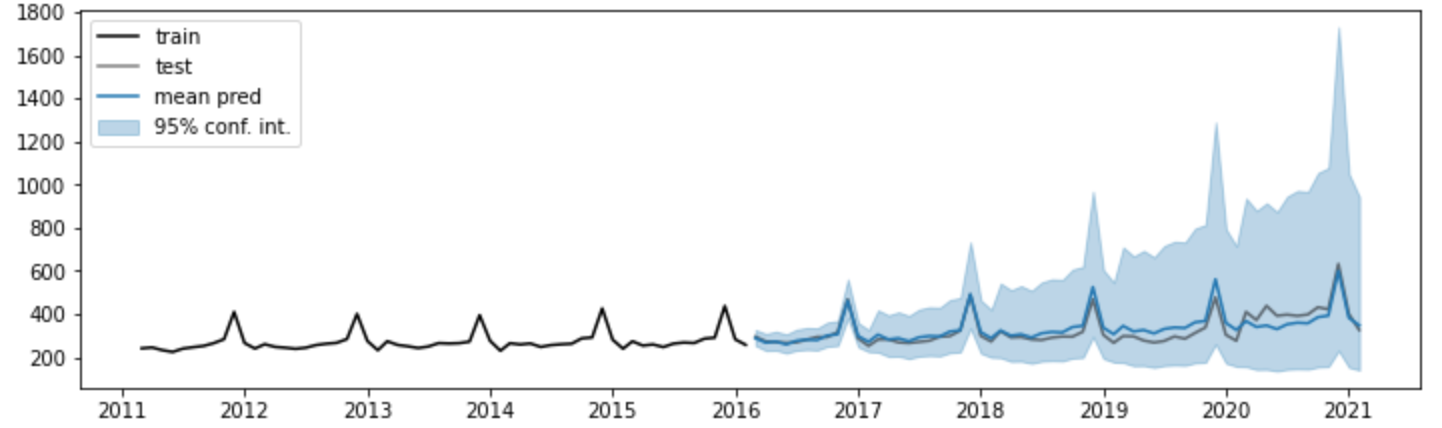
\includegraphics[width=0.8\textwidth]{var.png}
    \caption{Example of the forecast via VAR model}
    \label{fig:var}
\end{figure}

\begin{figure}[!ht]
    \centering
    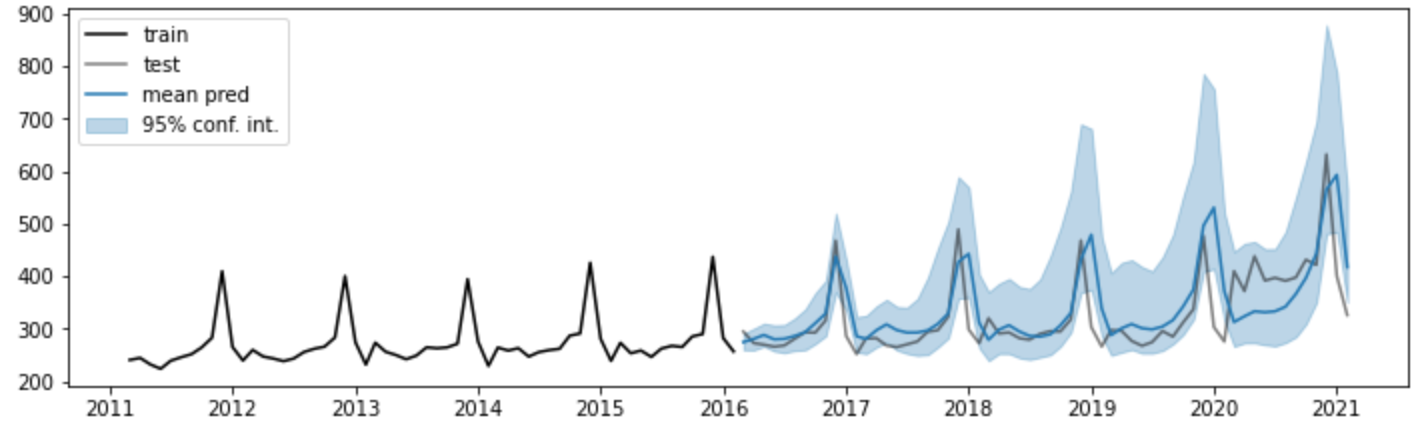
\includegraphics[width=0.8\textwidth]{transformer_realnvp.png}
    \caption{Example of the forecast via Transformer Real NVP model}
    \label{fig:transformer_realnvp}
\end{figure}

\begin{figure}[!ht]
    \centering
    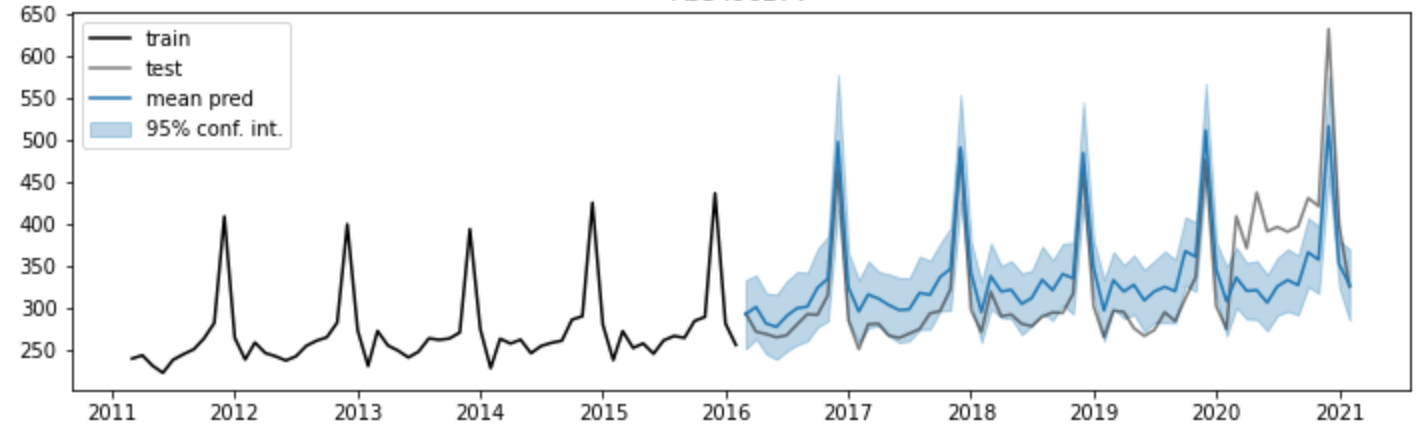
\includegraphics[width=0.8\textwidth]{gaussian_tcn.png}
    \caption{Example of the forecast via Gaussian TCN model}
    \label{fig:gaussian_tcn}
\end{figure}

\begin{figure}[!ht]
    \centering
    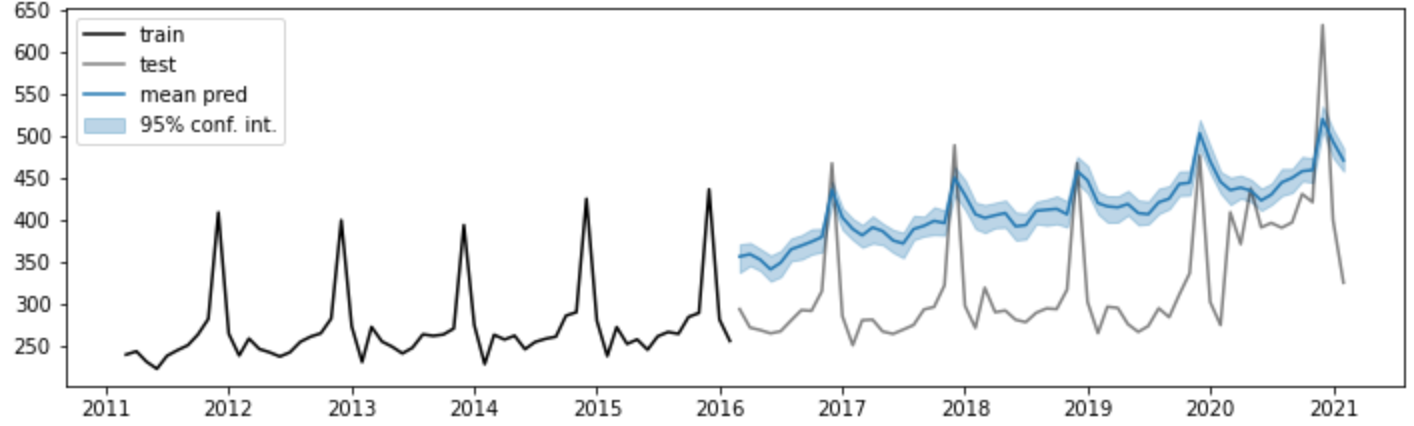
\includegraphics[width=0.8\textwidth]{tcn_cgan.png}
    \caption{Example of the forecast via TCN cGAN model}
    \label{fig:tcn_cgan}
\end{figure}

\begin{figure}[!ht]
    \centering
    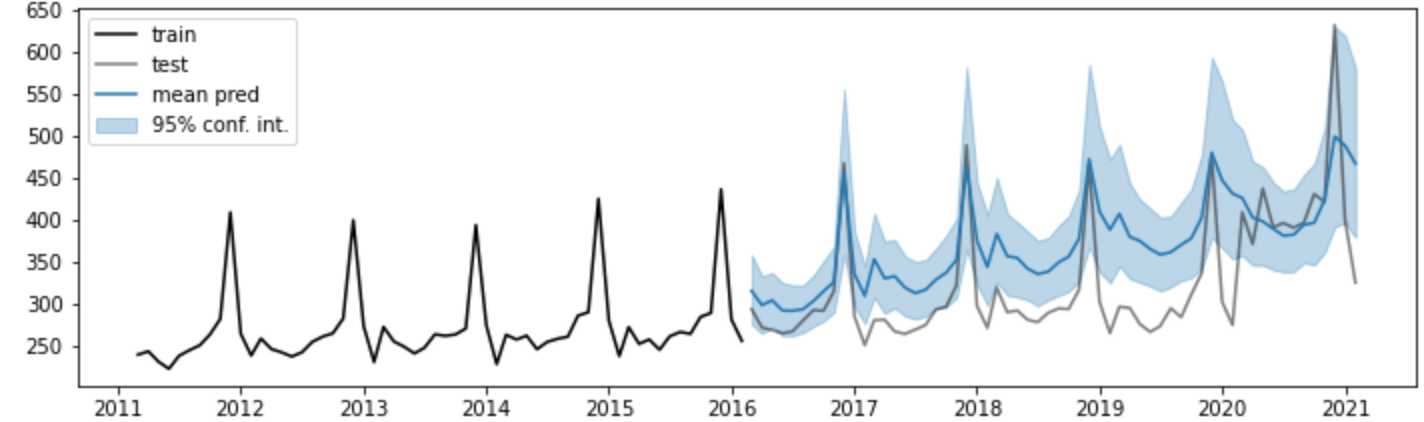
\includegraphics[width=0.8\textwidth]{vec_lstm.png}
    \caption{Example of the forecast via VEC-LSTM model}
    \label{fig:vec_lstm}
\end{figure}

The results obtained are shown in the table \ref{table:1}. As we can see, the best result for the QL metric was shown by the Gaussian TCN model, slightly ahead of the VAR model. At the same time, according to the CL metric, the Transformer Real NVP model was the best, slightly ahead of VEC-LSTM. According to the ACL metric, the Gaussian TCN model performed best. Examples of forecasts obtained from the models are in figures \ref{fig:var}, \ref{fig:transformer_realnvp}, \ref{fig:gaussian_tcn}, \ref{fig:tcn_cgan}, \ref{fig:vec_lstm}.

\section{Conclusion}

In this work, an attempt was made to generalize modern approaches to time series modeling. The classification of models was given by the type of modeling, as well as by the architecture of neural networks. The resulting review shows that deep generative models for the task of forecasting multivariate time series are actively developing at the present time, so it is likely that the number of such works will only increase in the near future. In addition, using such classification, we can combine the type of generative model and the architecture of the neural network, thereby obtaining new versions of the models. For example, in the literature, I have not yet come across variants of GAN with attention-based models, or TCN with Real NVP.

Despite the relative simplicity and efficiency of classical statistical approaches as VAR model, they have certain limitations. The complexity of such models increases quadratically with the number of time series components. Also, they do not take into account the complex nonlinear dependencies between the components of the time series. In addition, they are difficult to modify, for example, combining them with other models for general training. On the other hand, deep generative models have flexibility in customization and can take into account nonlinear dependencies. In addition, the use of data preprocessing techniques from classical statistical approaches can potentially improve the quality of deep models, which is a possible direction of study in this area.

\bibliography{main}

\end{document}
